\section{Architectural Design}
\subsection{Overview}
High-level components and their interaction. Informal view (free style notation), major
interfaces

\subsection{Component view}
Components + interfaces: component diagrams, composite structure, class diagrams (detailed view)
\begin{figure}[H]
    \centering
    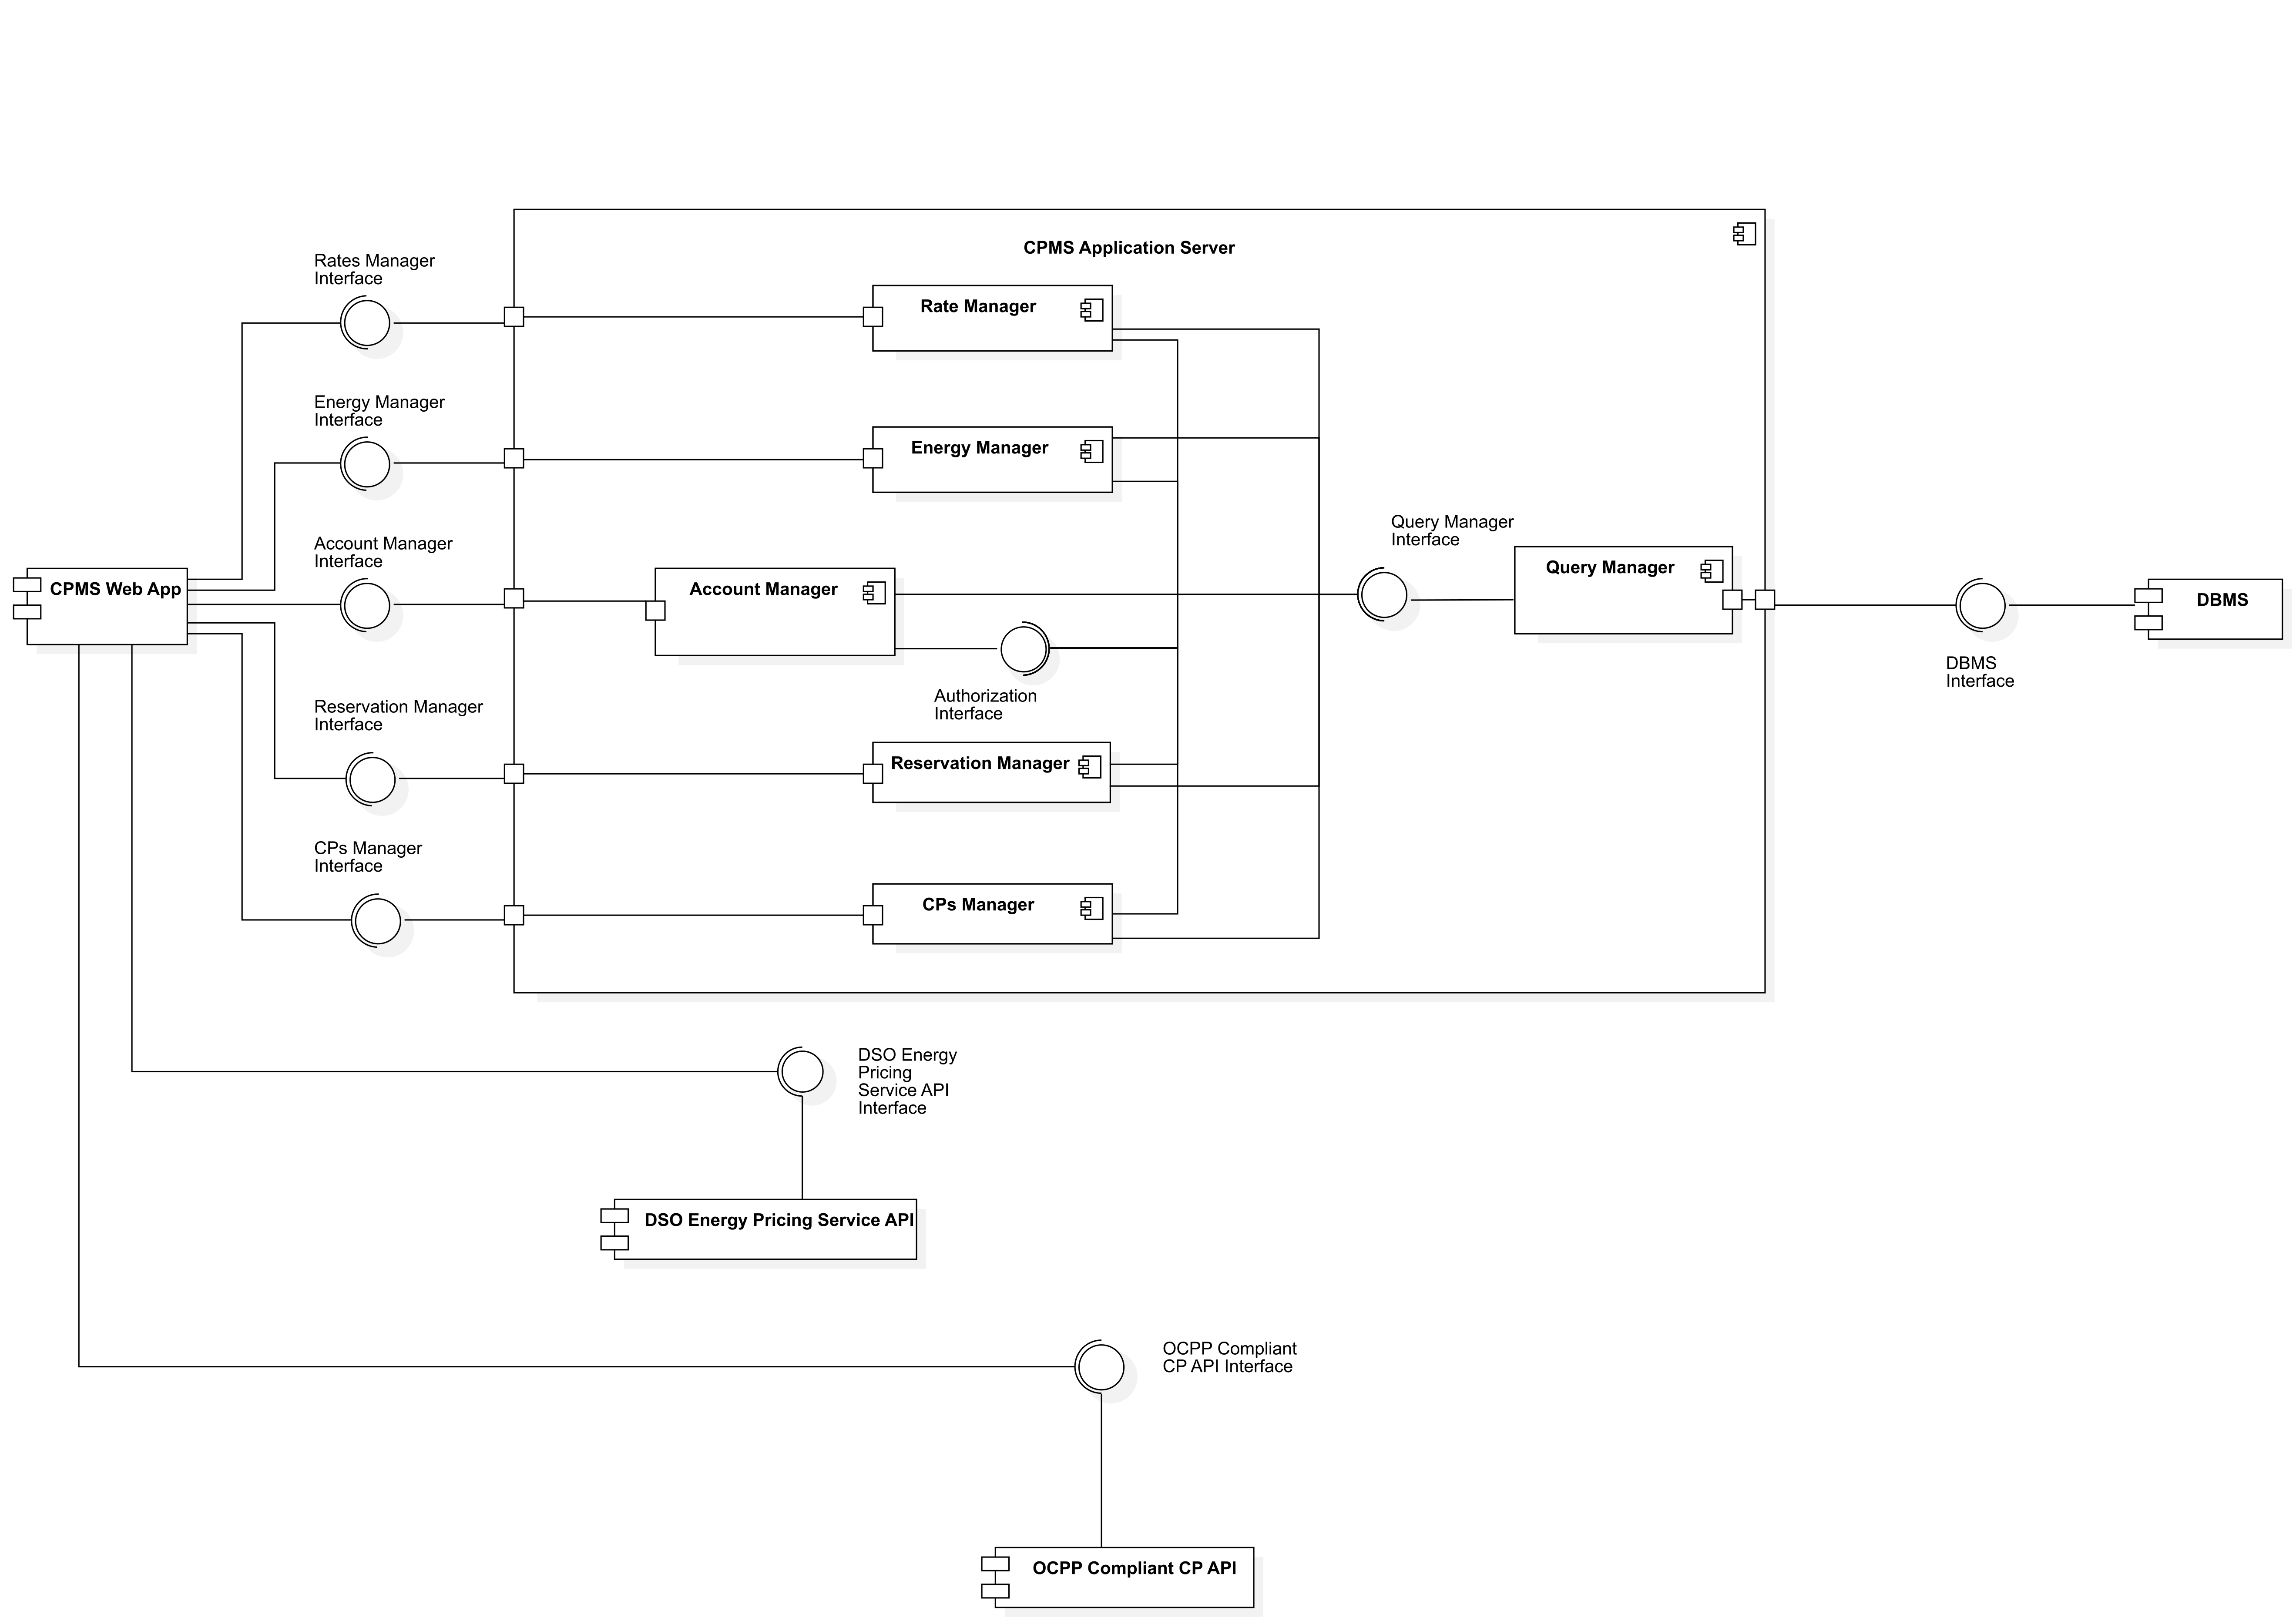
\includegraphics[scale=0.38]{src/ComponentDiagram/CPOdiagram.png}
    \caption{Charging Point Operator}
\end{figure} \vspace{1cm}

\subsection{Deployment view}
Infrastructure: deployment diagram(s) including non-logical elements (e.g., load balancer, firewall)
\subsection{Runtime view}
You can use sequence diagrams to describe the way components interact to accomplish specific tasks typically related to your use cases. Dynamics of the interactions: sequence
diagrams (realization of use cases)
\subsection{Component interfaces}
Details for each interface (name, signature, returned objects)
\subsection{Architectural Styles and patterns}
Please explain which styles/patterns you used, why, and how
\subsection{Other design decisions}